\documentclass[english]{textolivre}

% metadata
\journalname{Texto Livre}
\thevolume{18}
%\thenumber{1} % old template
\theyear{2025}
\receiveddate{\DTMdisplaydate{2024}{3}{20}{-1}}
\accepteddate{\DTMdisplaydate{2024}{4}{23}{-1}}
\publisheddate{\DTMdisplaydate{2024}{11}{29}{-1}}
\corrauthor{María Bobadilla-Pérez}
\articledoi{10.1590/1983-3652.2025.51692}
%\articleid{NNNN} % if the article ID is not the last 5 numbers of its DOI, provide it using \articleid{} commmand 
% list of available sesscions in the journal: articles, dossier, reports, essays, reviews, interviews, editorial
\articlesessionname{articles}
\runningauthor{Galán-Rodríguez; Bobadilla-Pérez; Barros-Grela}
%\editorname{Leonardo Araújo} % old template
\sectioneditorname{Hugo Heredia Ponce}
\layouteditorname{João Mesquita}

\title{Attitudes and perceptions: the role of artificial intelligence in the training of future secondary school foreign language teachers}
\othertitle{Atitudes e percepções: o papel da inteligência artificial na formação de futuros professores de línguas estrangeiras do ensino secundário}
\author[1]{Noelia Mª Galán-Rodríguez~\orcid{0000-0001-6662-7269}\thanks{Email: \href{mailto:noelia.galan@udc.es}{noelia.galan@udc.es}}}
\author[1]{María Bobadilla-Pérez~\orcid{0000-0002-4972-5980}\thanks{Email: \href{mailto:m.bobadilla@udc.es}{m.bobadilla@udc.es}}}
\author[2]{Eduardo Barros-Grela~\orcid{0000-0002-7533-5580}\thanks{Email: \href{mailto:ebarros@udc.es}{ebarros@udc.es}}}
\affil[1]{Universidade da Coruña, College of Education, Department of Specific Teaching Training and Research and Diagnosis Methods in Education, A Coruña, Spain.}
\affil[2]{Universidade da Coruña, College of Arts and Letters, Department of English, A Coruña, Spain.}

\addbibresource{article.bib}

\newcommand\subsubsubsection[1]{%
  \paragraph{#1}\mbox{}\\
}

\begin{document}
\maketitle
\begin{polyabstract}
\begin{abstract}
This study explores prospective foreign language teachers' attitudes towards integrating artificial intelligence (AI) into their teaching practices, focusing on the TWEE tool. Using a mixed-methods approach, data from 29 pre-service secondary school teachers in Spain were analyzed using SWOT analysis to assess TWEE's strengths, weaknesses, opportunities, and threats. Internal strengths include resource variety and practicality, while weaknesses involve interface issues and language constraints. External opportunities include quick activity creation, while threats center on ethical concerns and teacher redundancy risks. Despite concerns, participants generally express a positive attitude towards AI, acknowledging its potential to enhance written tasks, motivation, and technological literacy. Pedagogical implications underscore the need for a balanced AI integration approach, considering accessibility and ethical concerns. Further research is suggested to explore AI tool implementation in classrooms. This study contributes to understanding AI's role in language education and informs strategic planning for its integration.


\keywords{Foreign language teaching \sep Artificial intelligence \sep Secondary Education \sep TWEE \sep Pedagogical perspectives}
\end{abstract}

\begin{portuguese}
\begin{abstract}
Este estudo explora as atitudes dos futuros professores de línguas estrangeiras relativamente à integração da inteligência artificial (IA) nas suas práticas de ensino, centrando-se na ferramenta TWEE. Utilizando uma abordagem de métodos mistos, os dados de 29 professores de ensino secundário em início de carreira em Espanha foram analisados utilizando a análise SWOT para avaliar os pontos fortes, os pontos fracos, as oportunidades e as ameaças da TWEE. Os pontos fortes internos incluem a variedade de recursos e o carácter prático, enquanto os pontos fracos envolvem questões de interface e restrições linguísticas. As oportunidades externas incluem a criação rápida de atividades, enquanto as ameaças se centram em preocupações éticas e riscos de redundância de professores. Apesar das preocupações, os participantes expressam geralmente uma atitude positiva em relação à IA, reconhecendo o seu potencial para melhorar as tarefas escritas, a motivação e o letramento tecnológico. As implicações pedagógicas sublinham a necessidade de uma abordagem equilibrada da integração da IA, tendo em conta a acessibilidade e as preocupações éticas. Sugere-se mais investigação para explorar a implementação de ferramentas de IA nas salas de aula. Este estudo contribui para a compreensão do papel da IA no ensino das línguas e serve de base ao planeamento estratégico para a sua integração.

\keywords{Ensino de línguas estrangeiras \sep Inteligência artificial \sep Ensino secundário \sep TWEE \sep Perspectivas pedagógicas}
\end{abstract}
\end{portuguese}
\end{polyabstract}

\section{Introductioon}\label{sec-introduction}

Event journalism mainly contemplates homicides, traffic accidents, drug
trafficking and robberies. Also, suicides, accidental falls, and
drowning, although the same informative treatment is not always applied
to all of them \cite{olivar2020tratamiento}.

Among all these topics, traffic accidents prevail in terms of
information compared to the rest due to their practically daily
frequency, the victims, and deaths they generate, the spectacularity and
visual impact of the images and the social alarm they arouse
\cite{rodriguez2011informacion}.

Event journalism understood until now as \enquote{specialized journalistic
information that deals with a varied subject centered on the commission
of crimes, accidents, catastrophes and curious and surprising facts}
\cite[p. 2]{rodriguez2011informacion}, faces in the 21st century the challenge
of a new technological dimension that allows the possibility of
producing news through automated journalism \cite{jamil2021automated}. In this
sense, people are already beginning to talk about \enquote{Robot Journalism},
\enquote{Automated Journalism} and even \enquote{Cognitive Journalism} where Artificial Intelligence (AI) has begun to occupy a field traditionally dominated by the human factor in the management of organizations. Also, in the media and in society through the application of Data Mining, to generate
algorithms that allow automation of management and refer it to the work
of bots in the production of news \cite{tunez2020from}.

It may seem that the journalistic profession is seemingly oblivious to
the robotization of newsrooms, but the origin of mass automation dates
to 2015, when the Associated Press (AP) automatically generated 3,000
\enquote{corporate earnings} stories in the US each quarter (IMT, 2019).

The editorial line, the agenda setting itself and the political
orientations of each communication media generate differences in the way
of covering the news about accidents \cite{arce2017accidentalidad}, but, within the information of events, it seems that the media
have shown a preference for certain types of news and events \cite{duran2020responsabilidad}. Specifically, it is expected to find a greater
number of news items referring to traffic accidents compared to other
types of events.

The agenda-setting theory maintains that the media influence the issues
that concern and speak about citizens, that is, that they can shape the
public agenda, in this case making it easier for citizens to talk
preferentially about traffic accidents over other types of events
\cite{scheufele2007framing}.

When the media publishes a greater amount of news about traffic
accidents, readers are not only informed about it, but they are also
influenced to think and give their opinion on that topic. In other
words, the media have a certain capacity to establish the agenda of the
set of issues about which a society speaks or is debated at a given
moment \cite{mccombs1972agenda}. In this way, it is intended to influence
the construction of news and information that they send to the public
\cite{vos2015how}.

It is also intended to obtain an answer on whether this greater number
of news publications on traffic accidents responds to a rigorous
elaboration and with its own elaboration or if the media are limited to
automatically transferring the information, they receive from the
emergency services. The media are in permanent contact with these
services, which are the ones who send them the necessary information to
produce news about traffic accidents, but the immediacy and permanent
updating of this information affects their journalistic rigor,
especially in digital newspapers.

According to González Ortiz, head of the \enquote{events and courts section} of
\emph{Diario de Navarra}, the main sources are the emergency services
and the police (personal communication, October 24, 2018). Crime
reporters draw on a variety of sources including:
\begin{itemize}
	
\item The police (through their press offices);
\item News agencies (mainly from \emph{EFE} and \emph{Europa Press});
\item Those of authors, victims, and witnesses (important sources but
difficult to obtain);
\item The judicial ones (the event journalist is usually also a court
journalist);
\item Undetermined sources (with and without attribution);
\item Other sources (forensic, penitentiary, neighborhood, union, health,
state, regional or municipal administrations, the media or traffic,
surveillance, emergency, or relief services \cite{rodriguez2015manual}.
\end{itemize}

Among all of them, journalists resort more frequently as a source of
information to prepare news about events to the police sources, which
include the National Police Corps, Local Police and Civil Guard, which
are the ones that make up the Security Forces and Corps of the State, as
established in Organic Law 2/1986, Security Forces and Corps (1986).
There are also specific services in each autonomous community.

The general objective of this study is to analyze the similarities
between news about traffic accidents (headlines and complete
journalistic pieces) published in different digital media.

The following are proposed as specific objectives:

Obtain information about the existence and repetition of exact news of
traffic accidents.

Obtain enough evidence to conclude that the media carry out a simple
dump of the news obtained from the emergency services and that,
therefore, there is an automated journalism model for the transmission
of news about traffic accidents.
\section{Theoretical Framework}\label{sec-theoreticalframework}

\subsection{Audio visual Translation and Didactic Audio visual Translation} \label{sub-sec-audiovisualtranslation}

As posited by \textcite{diaz-cintas2012subtitulos}, audio-visual translation (AVT) can be
defined as the process of transferring the cultural and linguistic
content of an audio-visual medium into another language. In doing so, it
is essential to consider the restrictions inherent to the medium in
question and to respect the original communicative purpose. Prior to
this definition, \textcite{diaz-cintas2009new} expounded that AVT had become a
crucial means of disseminating audio-visual content, not only on an
international scale, but also to ensure the accessibility of multimodal
content to diverse audiences.

The three principal modes of AVT are subtitling, dubbing and audio
description. In their study, \textcite{talavan2023didactic} define subtitling as the translation of a dialogue
into written form, text which is then placed at the base of the screen.
Moreover, dubbing entails the replacement of the original dialogue with
that in the target language, ensuring that the translated audio
syncronises with the movements of the actors' lips. As
a final point, audio description aims "to make the visual content of an
event accessible by conveying it into spoken words" \cite[p. 246]{ibanez2016audiodescription}.

Conversely, \textcite{talavan2019traduccion} defines Didactic audiovisual translation
(DAT) as the didactic application of AVT procedures to the teaching of
the L2. This researcher posits that DAT has its roots in the 1980s, when
researchers and scholars began to recognise the potential of this
approach to language teaching and started to incorporate subtitles as a
tool in language laboratories. Furthermore, \textcite{fernandez-costales2023tradilex} add that students must utilise technology (new tools
available on the internet) and employ the specific strategies associated
with each mode.

As early as 2009, \citefirstlastauthor{diaz-cintas2009new} emphasised the significance of DAT in L2
instruction, noting that it enables learners to engage with native
speakers' productions, thereby facilitating a more
genuine encounter with the L2 and its associated culture. In this way,
DAT has demonstrated to be an effective tool, as it engages learners by
providing them with authentic audio-visual materials, which allows to
immerse themselves not only in the language, but also in the target
culture. \textcite{fernandez-costeles2021} concurs with this assertion, having
conducted research into the effects of DAT on the learning of the L2 in
a primary education environment.

Additionally, \textcite{chaume2018audiovisual} emphasised that this approach facilitates a
more profound comprehension of the L2 through the combination of
auditory and visual input, thereby enabling learners to discern the
authentic, natural usage of language by native speakers. In this regard,
\textcite{gonzalez-vera2016audiovisual} illustrate that DAT facilitates more
effective learning by offering immediate feedback on pronunciation and
grammar, promoting more rapid language development.

\subsection{Didactic Dubbing and Subtitling}\label{sub-sec-didacticdubbing}

The combination of didactic dubbing and subtitling facilitates the
integration of the four linguistic skills. The primary focus of dubbing
is on oral skills, namely listening comprehension and speaking, whereas
subtitling is more closely aligned with written skills, namely reading
comprehension and writing. In addition to the aforementioned skills, we
can include the fifth skill, translation \cite{Carreres03072017}.

Regarding dubbing, \textcite{diaz-cintas2012subtitulos} mentions that students benefit
from exposure to a diverse range of dialects and accents. Furthermore,
it capacitates learners to enhance their oral comprehension and speaking
abilities concurrently, while fostering motivation through the
incorporation of a multimodal component. Moreover, it facilitates the
acquisition of the L2 in an authentic and natural manner
\cite{fernandez-costales2023tradilex}, as students engage with
genuine oral language in authentic contexts, diverging from the
structured materials typically provided in textbooks.

The benefits of subtitling have also been the subject of academic
investigation. \textcite{ÁlvarezSánchez_2017} asserts that the utilisation of
subtitles not only fosters the development of linguistic skills but also
upgrades the comprehension of paralinguistic and cultural elements. It
also encourages self- and cooperative learning, with learners at the
core of the learning process. Likewise, she explains that audiovisual
media reflects a multitude of communicative scenarios, thus facilitating
comprehension of an oral language text through the utilisation of
non-linguistic elements. Adding to this, \textcite{lertola2018translation} elucidates that
the advantages of employing subtitling are analogous to those of
translation. However, there is an additional benefit, as learners are
not merely translating a text from the source language to the target
language; they are also exposed to audiovisual material, which enables
them to observe and listen to authentic communication scenarios.
Additionally, \textcite{soler2020} states that subtitling enhances
vocabulary acquisition, provides motivation, facilitates productive
abilities (specifically, speaking and writing), ameliorates the L1, and
strengthens attention skills. As will be demonstrated, these
characteristics are consistent with the communicative approach that is
intended in Spanish L2 curricula.

Two previous studies have examined the combination of dubbing and
subtitling in L2 classes. \textcite{talavan2015first} put forth an
implementation of reverse subtitling and dubbing with the objective of
"improving oral and written production skills, along with general
translation competence" \cite[p. 169]{talavan2015first}. Their approach yielded highly
promising outcomes in terms of language acquisition. Similarly,
\textcite{BELTRAMELLO_2019} conducted an in-class implementation in accordance
with the aforementioned parameters. In her conclusions, she states that
the combination of the two modes is effective because, in addition to
facilitating language acquisition, students are exposed to "pragmatic
phenomena" \cite[p. 106]{BELTRAMELLO_2019}. In the process of dubbing, learners are required to
direct their attention towards the objectives of the speaker and the
utilisation of specific expressions, rather than others. Furthermore,
students have the opportunity to practise pronunciation, intonation, and
some paralinguistic aspects of language, thereby improving their
fluency. According to this scholar, ``it seems to reveal an untapped
potential in the combination of subtitling and revoicing as an aid to
language learning that offers abundant possibilities to practice and
develop different areas of language competence, such as pragmatic
competence'' \cite[p. 6]{BELTRAMELLO_2019}.

In light of the above, it can be posited that working with both DAT
modes concurrently represents an effective pedagogical approach. This
combination capacitates learners to simultaneously develop their
comprehension and production skills. Additionally, it improves
motivation, as students engage in a multimodal environment with
controlled exposure to authentic language usage in authentic contexts.

\subsection{The Montessori Method}\label{sub-sec-themontessorimethod}

The aim of developing innovative pedagogical approaches that align with
the needs of learners can be traced back to the 19th century. In
conjunction with the advent of new psychological theories, scholars
understood the necessity for a more individualised approach to teaching,
with a focus on the needs of the learner. Among the approaches that
emerged in this context were the Montessori Method or the Scientific
Pedagogy method, which was based on Maria Montessori\textquotesingle s
observations that children were capable of learning independently,
without the direct supervision of adults \cite{pla2007}.

\textcite{lillard2013playful} points that the Montessori Method is an educational
approach with the aim of promoting the holistic development of the
child. Its fundamental premise is the belief that children are innately
inclined towards learning. Consequently, educators must establish an
engaging and nurturing setting, provide individualized guidance through
experiential learning opportunities and encourage self-directed learning
by means of a blend of autonomy, suitable educational resources and
self-discipline \cite{marshall2017montessori}. Moreover, \textcite{pla2007}
assert that this method is founded upon four principal tenets: preparing
children for life, fostering a conducive learning environment,
refraining from undue interference in the learning process, and
providing sensorial materials to improve sensory development.

In addition, \textcite{marshall2017montessori} maintains that this method relies on the
development of two essential components: emotional and social skills.
The first seeks to ameliorate the emotional skills that help children
cope with the challenges of everyday life. The second focuses on
cooperation, empathy and mutual respect among students, and is performed
by activities which require cooperation. This way, learners build
relationships with their peers.

\textcite{montessori1937metodo} challenged the prevailing pedagogical trends of the
time, advocating for a teaching approach that empowers children to learn
through independent action. She emphasised the importance of educators
obtaining precise and logical observations of children, which serve as
the foundation for their instructional decisions. Accordingly, the
pedagogical approach is founded upon exploration and discovery, wherein
pupils progress within a tranquil, respectful, and structured milieu
with the objective of fostering autonomy. This signifies a shift in the
role of the teacher, moving from a director who oversees both
children\textquotesingle s learning and behaviour \cite{denervaud2019} to a supportive figure who establishes a
nurturing environment, in which pupils are able to flourish and reach
their full potential \cite{marshall2017montessori}. Pupils are encouraged to work
independently at their own pace in an environment replete with tangible
materials designed to promote discovery, exploration, and, most
crucially, creativity \cite{marshall2017montessori}. \textcite{denervaud2019} emphasise the necessity for these materials to be
self-correcting, thus enabling children to learn through trial and
error.

Additionally, \textcite{pla2007} claim that it is imperative
to respect the rhythms of pupil growth, requiring that teachers adapt
the content and devise individualised plans in accordance with the pace
of each child. Moreover, the aforementioned plans must be aligned with
the child\textquotesingle s interests, while also fostering
self-discipline. Furthermore, the learning proposals must develop five
key aspects: practice, imitation, repetition, classification and order.

It is therefore necessary to implement changes to the layout of the
classes and the grouping of the pupils. In the first case, \textcite{pla2007} explain that the classrooms must be reorganised, with the
elimination of desks, banks and class platforms for teachers, and the
adaptation of furniture to the height and strength of children. This
signifies that the classrooms are constituted as a structured framework,
which facilitates access to the materials and delineates specific spaces
to play, speak, rest and listen. Secondly, \cite{lillard2013playful} points that
pupils should be distributed in mixed-age classrooms, separated by a
range of three years: infants to three-year-olds, three to
six-year-olds, six to nine-year-olds, and from nine to twelve-year-olds.

This approach is founded upon the premise that children learn through
active engagement \cite{pla2007}. Consequently, didactic
workshops represent an efficacious instrument for the organisation of
educational activities. Among the advantages is the fact that workshops
facilitate hands-on teaching, which helps to maintain
students' interest and attention. Moreover, workshops
can be tailored to the specific abilities and requirements of each
pupil, thereby optimising the learning process. Additionally, workshops
facilitate teamwork and creativity, as children can engage in
collaborative activities. Nowadays, these learning environments have
evolved to encompass both physical spaces, such as science laboratories
or kitchens, and virtual environments. Nevertheless, the underlying
rationale remains consistent: learners engage in experiential learning
activities to apply the concepts they have acquired, thereby developing
the practical skills they will require in their future endeavours.

Moreover, this approach places an emphasis on the cultivation of
critical thinking abilities throughout the learning process \cite{murray2011montessori}. Pupils are encouraged to engage in exploration, discovery and
questioning to gain a deeper understanding of their surrounding
environment, which provides numerous opportunities for mutual assistance
\cite{pla2007}. The efficacy of this approach has been the
subject of considerable investigation, with \cite{lillard2013playful} demonstrating
its advantages in domains such as cognitive development, academic
achievement and self-discipline.

Some of the objectives of this approach are aligned with those of DAT.
On the one hand, both are based on the development of
students' thinking skills. According to \textcite[p. 214]{ghaffari2017montessori}, "the process of independent
problem solving creates self-confidence and critical thinking skills".
Translation is categorized alongside the highest order thinking skills,
according to Bloom's Taxonomy. Conversely, both methods
encourage collaborative work, as the majority of DAT activities are
conducted in pairs or groups. Lastly, both methods facilitate
learners' autonomy in learning, allowing them to work
at their own pace while the teacher serves as a guide, providing access
to learning resources.

\subsection{Spanish Legislation on Education and DAT}\label{sub-sec-spanishlegislationoneducationanddat}

The latest Law on Education \cite{lomloe2020} and the Organic Law on the
Foral Decree 67/2022 of the Foral Community of Navarre establish the
compulsory curriculum for all schools in the region. With some additions
due to the particularities of the Community, the latter specifies what
the former decrees.

In regard to the teaching of the L2, it is asserted that the focus
should be on the development of oral skills, with educators providing a
range of tools to facilitate student engagement with the content.
Moreover, educators must promote instrumental learning, which enables
learners to develop other competencies and meaningful learning, by
integrating the different competences in the execution of projects, so
that students solve problems cooperatively, what strengthens autonomy,
reflection and responsibility. Additionally, the L1 will be employed
solely as a support tool in the acquisition of the L2. Finally, learners
must allocate time on a daily basis to audio-visual communication and
the promotion of creativity and scientific inquiry.

The legislation requires educators to provide multiple tools to
encourage learner engagement. The world in which students live is
multimodal. Video clips, online games, films and TV series constitute
the majority of their leisure activities. It could therefore be assumed
that introducing these new languages into the classroom will make
learners feel more at ease, which will in turn improve their motivation
and, consequently, the acquisition of the L2.

Undoubtedly, DAT promotes instrumental learning as students work with a
variety of inputs, including text, audio and the cultural contexts of
multimodal texts, and have to manipulate the language in order to align
it with the image. In addition, it strengthens autonomy and reflection,
as learners can work independently or in collaboration with others,
which encourages them to problem-solve collectively and improves their
sense of responsibility. Finally, it integrates a range of competencies,
including linguistic communication, plurilingualism, digital
proficiency, personal and social skills, the capacity to autonomous
learning, consciousness, and cultural expressions \cite{Bobadilla-Pérez_CarballodeSantiago_2022,rodríguez-Arancón2023}, thereby implying
life-long learning, which is a fundamental aspect of the current
teaching and learning process.

Although the current legislation does not contemplate the use of the L1
and of translation in the class, \textcite{Carreres03072017,Colina03072017} have suggested that
translation should be considered as the `fifth skill', which ``can be
used as a pedagogical tool to integrate the original four skills to
enhance second language study'' \cite[p.~2]{Colina03072017}.

\section{Artificial Intelligence in Language Teaching}\label{sec-artificialintelligencein}
The integration of AI, particularly ChatGPT, in language teaching offers
numerous opportunities but comes with challenges that require thoughtful
consideration and strategic approaches. Teachers are encouraged to
embrace AI as a complementary tool, continually enhance digital
literacy, engage in human-machine collaboration, and shift towards
student-centered education to navigate the evolving landscape of
language teaching. \textcite[p.~167]{schmidt2022} discuss the
classification of key concepts in AI-powered language learning tools
scenarios as outlined by \textcite{baker2019}. They identify three
main categories:

\begin{itemize}
    \item Learner-facing AI tools: These tools are designed to assist students directly in improving their language skills. They typically incorporate features like practice patterns, feedback mechanisms, and drills aimed at enhancing comprehension and proficiency. An example cited is Babbel, an application that offers immediate feedback tailored to the learner's input, with a focus on areas such as mixed tenses and verb forms.
    \item Teacher-facing systems: This category encompasses tools intended to alleviate the burden on educators by automating various aspects of their work. These tools handle tasks such as grading assignments, providing feedback to students, managing classroom activities, and handling administrative duties. For instance, GradeScanner is highlighted as a tool capable of automatically grading multiple-choice tests, thereby saving teachers valuable time and effort.
    \item System-facing AI tools: These tools primarily serve institutional administrators or stakeholders by providing them with processed data. By analyzing data such as student transcripts and performance metrics, these tools offer insights that can inform strategic decisions at the institutional level. They may utilize algorithms to predict future student performance or identify trends within the learning environment, aiding in the development of effective policies and interventions.
\end{itemize}


\textcite[p.~119–120]{ravshanovna2023} discusses the benefits and drawbacks of
integrating AI into language teaching. AI offers personalized training
programs based on individual student needs, automates evaluation tasks
like grading essays and tests, and enhances feedback processes. It also
streamlines educational management and improves access to education,
particularly for remote learners through online courses. However,
challenges include AI's occasional lack of accuracy,
difficulty in adapting to diverse contexts, and limited ability to
interpret human emotions. Moreover, AI solutions may lack clarity and
struggle with creative thinking. Additionally, the implementation and
maintenance of AI systems require qualified personnel. While AI presents
opportunities for language teaching, it cannot entirely replace human
involvement, emphasizing the importance of balancing technology with
human intervention for optimal results.

The systematic review conducted by \textcite{sharadgah2022} provides a
comprehensive exploration of the literature on the integration of AI in
English Language Teaching (ELT) from 2015 to 2021. The review identifies
various AI applications in ELT, including automatic correction,
listening skill enhancement, oral training through AI-based robots,
machine translation, personalized teaching, and experimental studies
evaluating AI-based systems. While highlighting the positive impact of
AI on ELT efficiency and student satisfaction, the study also points out
challenges and gaps in the literature, emphasizing the need for clear
evaluation criteria and future research directions.

In a study by \textcite[p.~449]{hockly2023}, various AI-powered tools supporting
language development are discussed, such as Duolingo, Write \& Improve,
Grammarly, Google Translate, and chatbot apps. The focus is on the
effectiveness of chatbots, which have proven beneficial, especially for
lower-proficiency learners, offering clearly delimited contexts for
language practice. Despite some limitations, chatbots contribute to
improved learning confidence, motivation, and self-efficacy. Teachers
are encouraged to recommend chatbot apps for additional exposure to
English language content outside class time, enhancing overall learning
outcomes.

Moreover, \textcite[p.~78]{huang2023} highlight the extensive
opportunities presented by ChatGPT in foreign language teaching. For
learners, ChatGPT addresses limitations of traditional classrooms,
providing opportunities for communication, easy access to learning
resources, and individualized learning strategies. It fosters interest
in learning through interactive conversations. For teachers, ChatGPT
serves as a multifaceted tool, assisting in resource provision,
conversation practice, assessment, and virtual teaching. The combination
of teachers and AI tools is seen as a new model for effective teaching
and learning.

However, challenges identified by \textcite[p.~83]{huang2023} include
potential reductions in intercultural communication skills, the
weakening of self-correction abilities, difficulties in ensuring content
accuracy, concerns about cheating, and inherent limitations in AI tools.
To address these challenges, the authors propose teaching strategies,
emphasizing the acceptance of AI as a supportive tool, the importance of
continuous learning and digital literacy, human-machine collaboration,
and a shift towards student-centered, competency-focused education.
\section{Methodology}\label{sec-methodology}
The use of ICT virtual resources and digital tools in ESP classes during
wartime has been studied through analysis of scientific and
methodological literature. This has allowed for the development of an
educational technology that can be implemented at all stages of the
learning process. Both in preparation for classes and during the
learning process, the specified technology can be used for explaining
new material, fixing errors, repeating information, checking for
understanding, correcting mistakes, and summarizing learning material.
This approach allows for the principles of activity, interactivity, and
a dialogic style of education to be employed, while also combining
individual and group work. Additionally, it helps to maintain students'
psychological comfort, optimize the process of ESP learning, and develop
students' POECC. The ICT tools presented can be used to engage and
motivate students in online classes, diversify visual aids, and create
interactive educational materials for whiteboards. Despite the
challenges of wartime and remote learning, resources such as Skype,
Blogger, Teams, and Zoom enable the organization of individual group
work, communication with students, creation of various tasks, and
automatic evaluation of their completion. The described platforms have
several advantages, including the ability to use free versions,
accessibility from different browsers and devices, and an
easy-to-understand interface that demonstrates the
tool\textquotesingle s capabilities. A\textbf{ }variety of content and
formats, including tests, quizzes, puzzles, crosswords, games, mind
maps, and diagrams in Kahoot, Quizizz, Quizlet, Learning Apps can
help to prevent the monotonous repetition of typical exercises. Students
can create their own organizers and bookmarks using tools such as
Padlet, Evernote, and Pinterest. Effective visual aids for presenting
learning material include Canva, Prezi, Maze, and Row Toon. The online
platforms Dropbox, Padlet, Pinterest, and Penzu enable users to share
their work and ideas. Students do not always have access to a computer,
so using platforms via mobile phones allows them to complete
tasks anywhere and without special technical requirements.

\subsection{Criteria}\label{subsec-criteria}
According to the theoretical analysis of the development of the POECC in
the motivational, cognitive, operational, and creative spheres of the
pre-service teachers of mathematics identified the following criteria:
motivational, cognitive, operational, and creative. Due to the specified
criteria, the development of POECC was assessed during the pre- and
post-stages of the experimental training of using ICT technology in ESP
learning. Table 1 presents the main criterion characteristics and
indicators.

\begin{table}[!htpb]
%\renewcommand{\arraystretch}{1.5}
\centering
\caption{POECC development criteria \cite{dmitrenko2020autonomous}.}
\label{tab-01}
\begin{threeparttable}
\begin{tabular}{l p{5cm} p{7cm}} 
\toprule
\emph{Criterion} & \emph{Characteristics of the criterion} & \emph{Indicators of the criterion} \\
\midrule
Motivational & ensures involvement in professional activity. It represents the positive attitude toward pedagogical creativity, awareness of the importance of POECC, which is revealed in satisfaction with the teaching profession, a desire for self-education, and active participation in work. & the desire to acquire knowledge, and improve	ESP skills; awareness of personal meaning and significance of	professional self-improvement; formation and orientation of the need for	POECC, self-education, and professional development; formation of motives; interest in ESP, intercultural knowledge, and skills; motivational interest in the chosen specialty. \\

Cognitive & is defined as a system of acquired knowledge and skills including purpose, principles, content, methods, techniques, and organizational forms of educational activities. & the completeness, correctness, and quality of the application of theoretical knowledge; the ability to select, process, and systematize ESP information; experience in recognizing norms of professional expression; free use of the thesaurus of professional terms; understanding and producing English texts related to the specialty. \\

Operational & is the appropriate application of POECС; as well as the ability to manage the educational process and one's own development. & the initiative, organization, self-discipline, self-control, productivity, the level of POECC, the presence of professional thinking, and the ability of self-education, etc. \\

Creative & describes the level of creativity and personal qualities of pre-service mathematics teachers, as well as their ability to think creatively, develop, analyze, and assess their readiness for professional activities in English for Specific Purposes (ESP). & the	ability to structure the process of solving educational tasks, outline the stages; correlate methods with types of tasks; self-control and adjust further activities; compare expected and obtained results; correlate practical experience and theoretical information. \\
\bottomrule
\end{tabular}
\end{threeparttable}
\source{\cite{dmitrenko2020autonomous}.}
\end{table}

Based on the given criteria, the pre-service teachers of mathematics were classified into three levels of POECC development: low, medium, and high (\Cref{tab-01}).

	\begin{table}[!htpb]
	\centering
	\caption{POECC development criteria \cite{dmitrenko2020autonomous}.}
	\label{tab-02}
	\begin{threeparttable}
    \begin{tabular}{ l p{4cm} p{4cm} p{4cm}}
    \toprule
	\emph{Criterion/Level} & \emph{Low level} & \emph{Medium level} & \emph{High level} \\
	\midrule
	Motivational & The student may not fully appreciate the personal and
				social importance of professional activity in ESP. They may not feel a
				strong need for it and may even view it negatively. As a result, they
				may only engage in ESP professional activity when required and may not
				demonstrate long-term commitment or independence. & The student is aware
				of the importance of professional activity in ESP formation of
				professional qualities, and willingly participates in it, shows positive
				emotions, quite active and independent in solving typical tasks but
				often requires a teacher's help. & The student clearly expresses
				persistent interest in ESP professional activity, eagerly 
				participates in it, shows responsibility, strives for independence and
				leadership, and actively shows positive emotions. \\
				Cognitive & The student has a limited understanding of ESP, recalling
				only basic concepts from memory and often misunderstanding their
				essence. They possess some ideas about the structure and methods of ESP
				professional activity, but these are not fully developed. & The student
				demonstrates an understanding of the role of ESP professional activity
				and possesses the necessary knowledge to explain, retell, and provide
				specific examples. However, there are some inaccuracies in their
				application of this knowledge when performing typical tasks. & The
				student has a fairly fluent command of terminology, can give accurate
				definitions and characteristics of concepts, clearly distinguishes the
				activity stages, passes existing knowledge, and applies it in new
				conditions to perform atypical tasks. \\
				Operational & The student is partially aware of the content of ESP
				professional activity and its operational composition, begins to carry
				it out, can report on his / her actions but cannot organize his / her
				actions without outside help, and cooperates with others quite
				successfully. & The student consciously and independently performs
				previously learned ESP professional activity in a typical situation and
				knows how to identify the inconsistency of a new task and a learned way
				of acting. & The student performs ESP professional activities quite
				fluently, is aware of each step, critically evaluates his / her actions
				at all stages, and can change a well-known method of action or build a
				new one to perform a non-typical task. \\
				Creative & The student uses the semi-patterned activity and the
				primitive tools, stays within the given or initially found method of
				action, and does not see alternative ways of performing the task. & The
				student looks for alternative solutions in a typical situation,
				independently combines known methods, analyses the task conditions, and
				is ready to describe the cause of difficulties or a new method. & The
				student freely applies acquired knowledge and a method of activity in
				non-standard situations, offers alternative ways of solving tasks, and
				reasonably chooses the optimal one. \\
				\bottomrule
            \end{tabular}
		\end{threeparttable}
		\source{\cite{dmitrenko2020autonomous}.}
	\end{table}

In the process of implementing developed technology, virtual resources,
and digital tools were used in the experimental ESP online training of
pre-service teachers of mathematics.

In order to provide free access, a resource center of teaching materials
intended for use by students was created. It was placed on a separate
page of the teacher's website \enquote{English for Students of Mathematics}.
The site page contained placement tests, current and intermediate
control tests; thematic texts, speech and language exercises; texts on
specialty for annotation and summary; an electronic manual; additional
materials: an English-Ukrainian mathematical dictionary, examples of
reading mathematical expressions, tips for writing annotations and
summaries, tips for choosing and using learning and communication
strategies, etc. (\Cref{fig-01}).

\begin{figure}[htpb]
\centering
\begin{minipage}{.65\textwidth}
\caption{Website page of ESP for pre-service teachers of mathematics.}	
\label{fig-01}
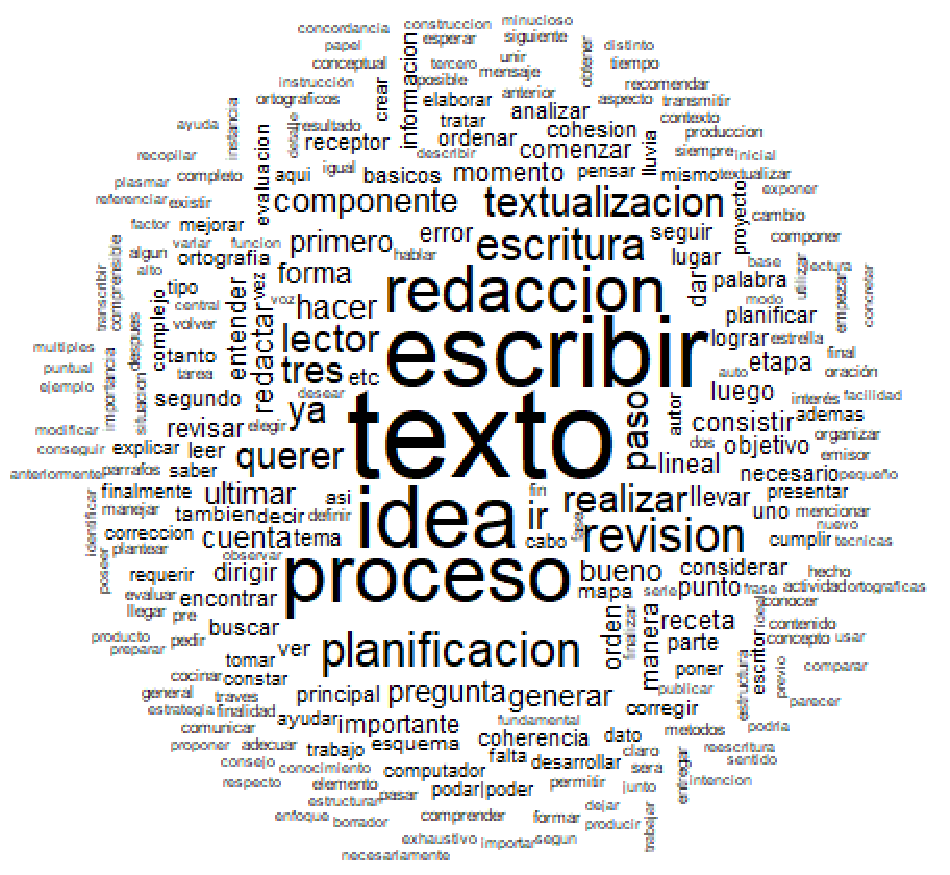
\includegraphics[width=\textwidth]{figure01}
\source{\cite{dmitrenko2020autonomous}.}
\end{minipage}
\end{figure}
The created e-textbook allowed the students to \begin{enumerate*}[label=\arabic*)]
	
	\item practice professional
	lexical skills; 
	\item carry out current control of the understanding of the
	content of the text on the specialty; 
	\item communicate using the learnt
	professional vocabulary; 
	\item discuss educational and professional problem
	situations; 
	\item prepare public speeches on a number of professional
	issues; 
	\item search for new textual, graphic and audio professionally
	oriented English information and analyze it; 
	\item write professional
        letters and documents in English (\Cref{fig-02}).
\end{enumerate*}

\begin{figure}[htpb]
\centering
\begin{minipage}{.65\textwidth}
\caption{Screenshot of the page (listening to the dialogue) of the e-textbook \enquote{Mathematics}.}	
\label{fig-02}
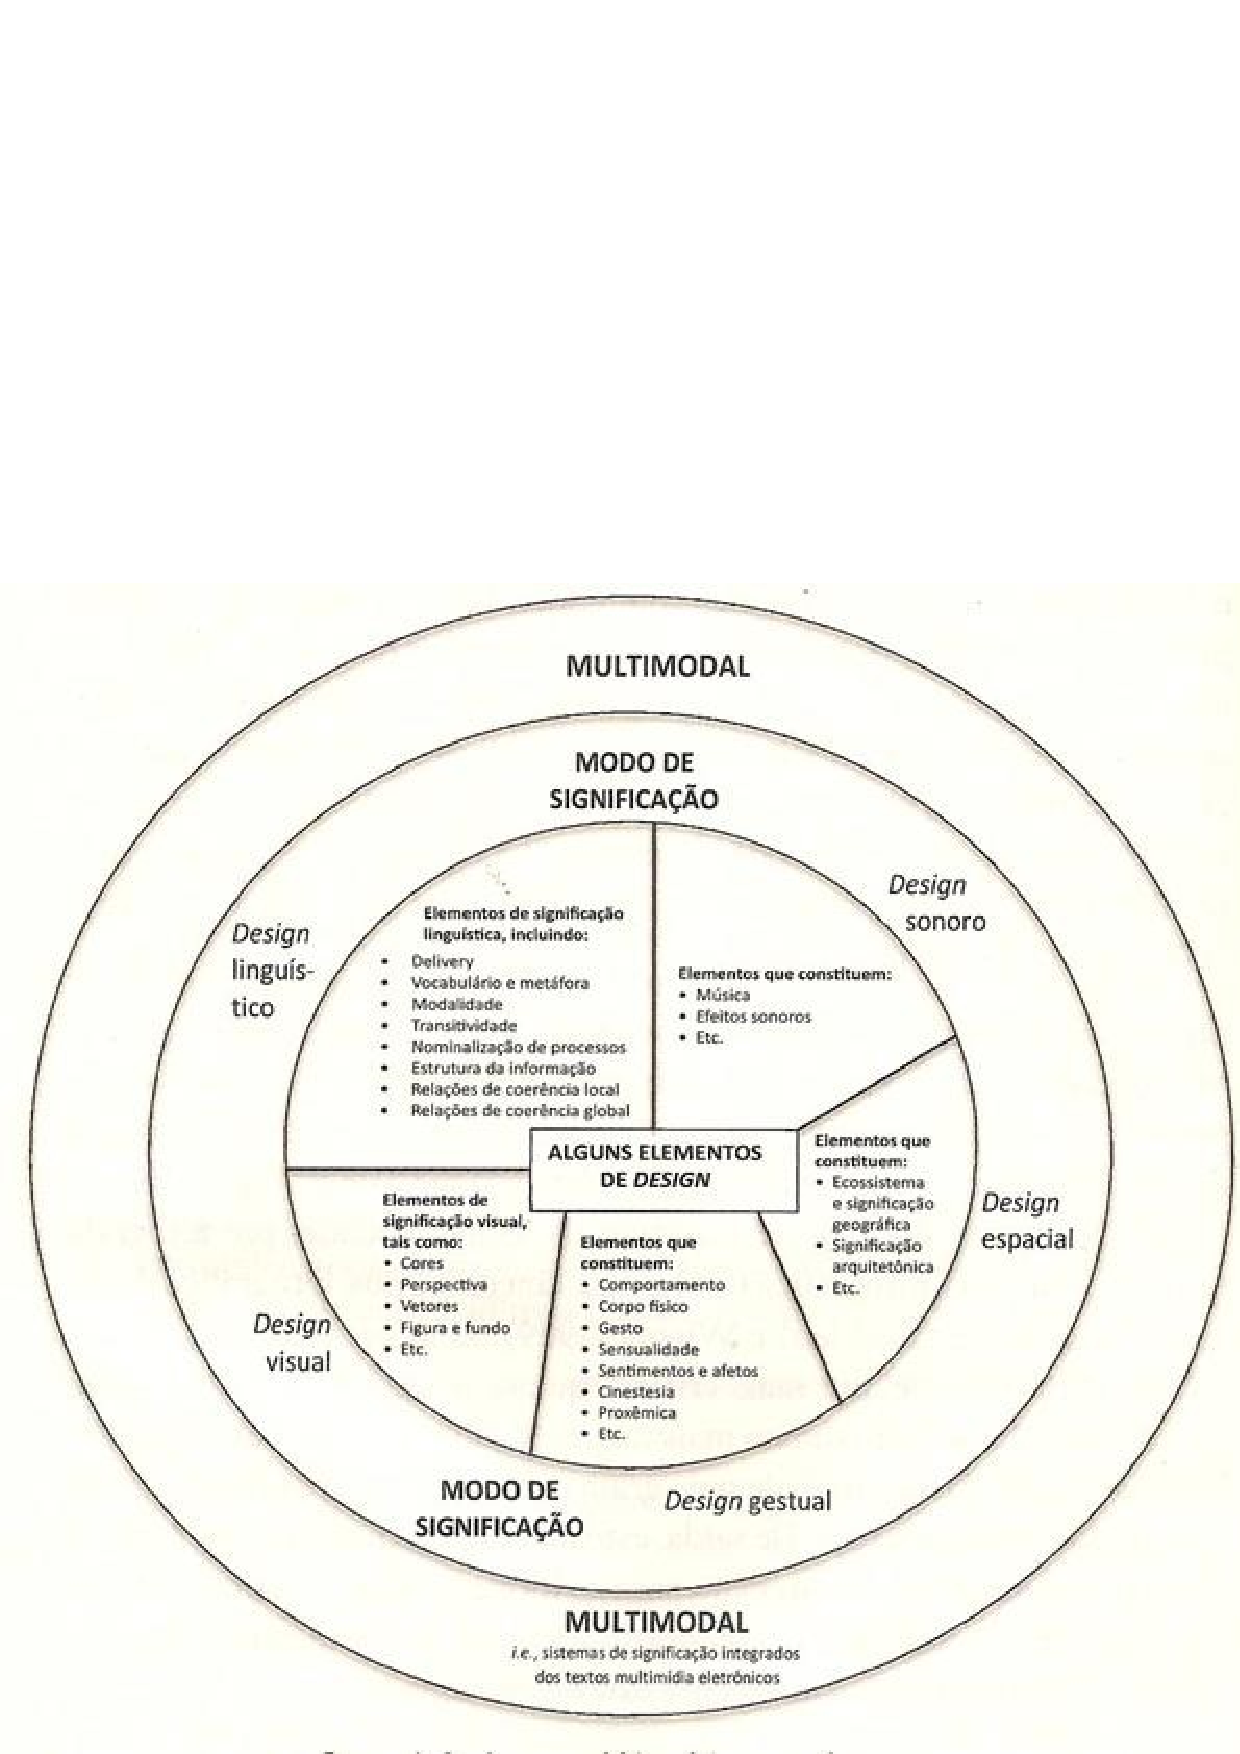
\includegraphics[width=\textwidth]{figure02}
\source{\cite{dmitrenko2020autonomous}.}
\end{minipage}
\end{figure}

Various applications have been used for interactive online ESP classes.
For example, the universal designer of interactive tasks
LearningApps.org was used to support the ESP learning process with the
help of interactive modules. Both the teacher and the student could
create interactive tasks based on ready-made templates. Such
verification and consolidation of the students' knowledge in a playful
way contributed to the formation of their cognitive interest in the ESP
educational component. The service included a gallery of publicly
available interactive tasks in English and all learning materials might
be posted publicly or for private use. An effective mobile web-based
learning application for ESP classes Quizlet was used to study and
repeat lexical and grammatical material with the help of self-made
flashcards, which contributed to the rapid assimilation of English
training material. The Quizlet Live application allowed students to
check the quality of the learned lexical material in an individual or
group format. The Kahoot!, was used to create tests, games, and quizzes
and is freely accessible from any browser on any device with internet
access. The teacher could create (or use a database of ready-made ones)
interactive tests, lead discussions, and present other learning
materials. Some examples of applications for creating exercises are
presented below.

\textbf{Example 1}. The purpose of the exercise is to acquaint students with the
typical features of using computers, to check the level of understanding
of the text, and to read silently (intensive reading). Instructions:
\enquote{Follow the link. Read the first paragraph of the text and write the
title. Check the correct answer by clicking on the button \enquote{Check
your answer}. Click on the arrow and move to another paragraph. You
have 15 minutes to do this} (\Cref{fig-03}).

\begin{figure}[htpb]
\centering
\begin{minipage}{.65\textwidth}
\caption{An example of an exercise in the application Learning Apps.}	
\label{fig-03}
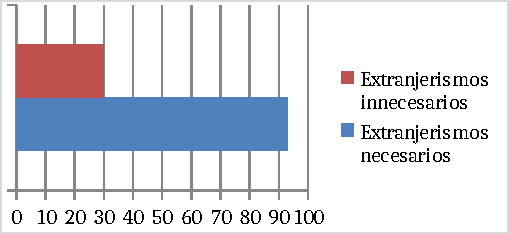
\includegraphics[width=\textwidth]{figure03}
\source{\cite{dmitrenko2020autonomous}.}
\end{minipage}
\end{figure}

\textbf{Example 2}. The exercise aims to check the level of understanding of
lexical items from the text. Instructions: \enquote{Follow the link. Match the
word with its definition. While doing the task, you will see the timer
which will count the time you have to complete the exercise. If you
choose the wrong answer, the time will be doubled. The person who
completes the task the fastest gets the highest score} (\Cref{fig-04}).

\begin{figure}[htpb]
\centering
\begin{minipage}{.65\textwidth}
\caption{A sample of an exercise in the Quizzlet application.}	
\label{fig-04}
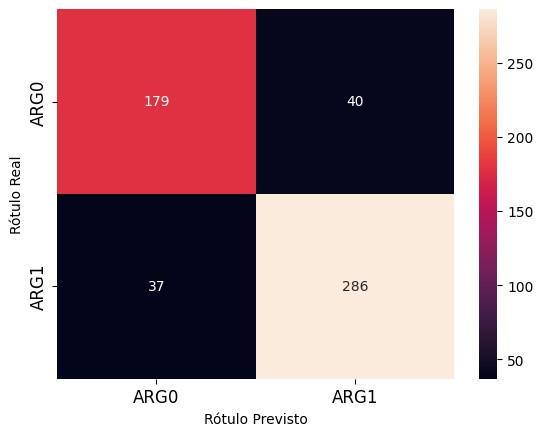
\includegraphics[width=\textwidth]{figure04}
\source{\cite{dmitrenko2020autonomous}.}
\end{minipage}
\end{figure}

\textbf{Example 3}. The purpose of the exercise is to check the level of reading
comprehension and text analysis. Instructions: \enquote{Take your mobile
phone and follow the link (\url{https://kahoot.it/}). Ask your teacher
for the code, enter it and your name. On the teacher's screen, you will
see the fact about computers and two sentences with red and blue colors.
Read the fact and choose the right color for yourself on the phone. If
you already know the fact, then you are doing great. If you don't know
the fact, then explain what exactly you want to discover about it. The
one who shares the opinion the most of all will get the highest score}
(\Cref{fig-05}).


\begin{figure}[htpb]
\centering
\begin{minipage}{.65\textwidth}
\caption{An example of an exercise in Kahoot!}	
\label{fig-05}
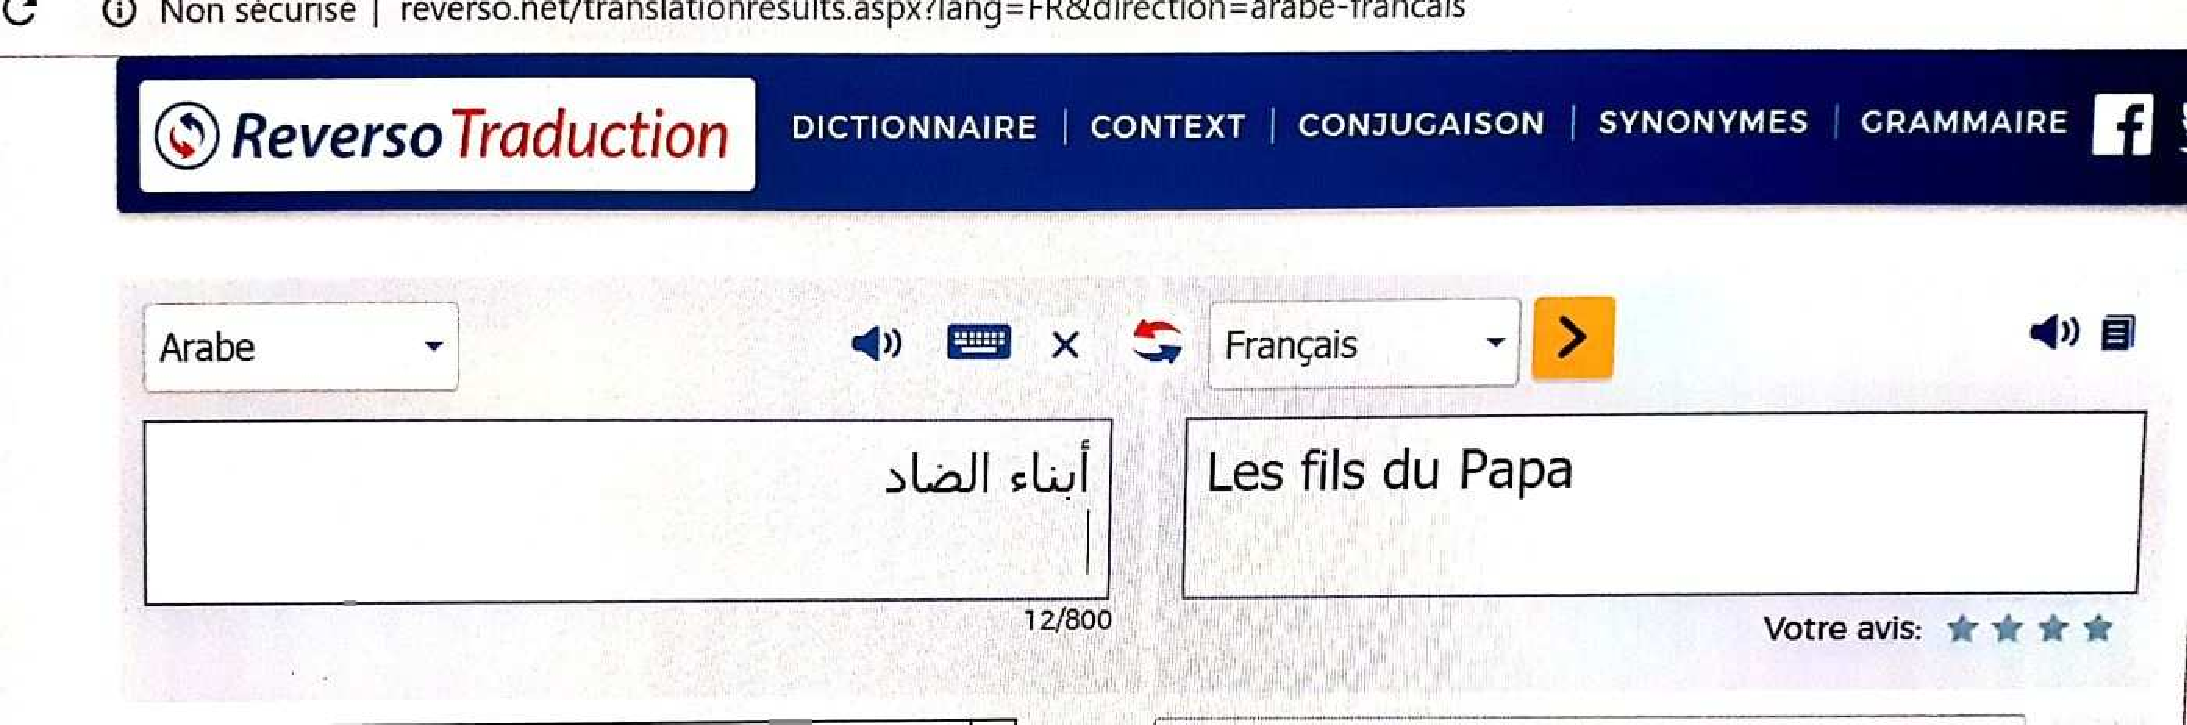
\includegraphics[width=\textwidth]{figure05}
\source{\cite{dmitrenko2020autonomous}.}
\end{minipage}
\end{figure}

\subsubsection{Participants}\label{subsubsec-participants}

The pre-service teachers of mathematics were divided into two
homogeneous groups: the control group (CG) – the formation of POACC
under usual conditions and the experimental group (EG) – the formation
of POACC under the influence of an active pedagogical factor – with the
use of virtual resources and digit tools. The participants of the study
were second-year students of the specialisation \enquote{Secondary Education.
Mathematics}, and \enquote{Mathematics} at the Faculty of Mathematics,
Physics and Computer Sciences, Vinnytsia Mykhailo Kotsiubynskyi State
Pedagogical University. The total number of participants was 100
students, 50 participants in CG and EG respectively. The experimental
training was carried out during one semester (17 weeks), and the ESP
classes were held twice a week. The ESP classes were held synchronously
online and lasted 80 minutes. Students were informed about the goals,
tasks, and conditions of experimental training and participated
voluntarily.

\subsubsection{The Study Stages}\label{subsubsec-thestudystages}

The study on the appropriateness of using ICT technology in ESP learning
by pre-service teachers of mathematics consisted of three stages. The
task of the \emph{first} stage was to measure the level of development
of the POECC of pre-service teachers of mathematics in EG and CG at the
beginning of the experimental training. The task of the \emph{second}
stage was to carry out the actual experimental training of ESP in EG
using the developed technology of ICT with virtual resources and digital
tools, and traditional training (without ICT tools) in CG. The task of
the \emph{third} stage was to diagnose and compare the level of
development of POECC of pre-service teachers of mathematics in CG and EG
after the introduction of an active pedagogical influence factor,
namely, the educational technology of using ICT in ESP learning.

\subsubsection{Instruments}\label{subsubsec-instruments}

The students' level of POECC was measured at the beginning and after the
experimental training (pre- and post-phases). The test was administered
to the students to assess the development of POECC according to the
following learning outcomes, which included 4 parts: \begin{enumerate*}[label=\arabic*)]
\item  knowledge of
basic English professional terms; 
\item the ability to translate
professional texts; 
\item the ability to analyze the content of English
professional sources; 
\item the ability to listen and understand the oral
professional speech.
\end{enumerate*}

The evaluation was carried out by experts (English teachers) on a
100-point scale for four components: knowledge of basic English
professional terms, translation of professional texts, content analysis
of English professional sources, and the ability to listen to oral
professional speech. Each component was evaluated in terms of 25 points.
The maximum level of development of each component was estimated at a
maximum of 25 points; the possible minimum was 1 point. The total score
for all components determined the level of development of the POECC of
pre-service teachers of mathematics: a low level – from 4 to 40 points;
an average level – from 41 to 74 points; and a high level – from 75 to
100 points. The assessment was carried out according to the
methodological recommendations of a group of experts.

The initial part of the test assessed the participants' understanding of
fundamental mathematical terms in English. The task required the
translation of fifty English terms, with each correct answer being
awarded two points. The second part of the test evaluated the students'
ability to translate professional English texts from English into
Ukrainian. Students were given to read and translate an English
professional text on a mathematical topic. The third part of the test
assessed students' capacity to analyze professional English sources and
select the appropriate section for further detailed study, analysis, and
use in pedagogical practice. The fourth part of the test evaluated
students' ability to comprehend spoken English in a professional
context. They were required to listen to a professional English text and
translate it into Ukrainian.

To assess group homogeneity and result reliability, we performed
statistical processing on the data using Pearson's $\chi^2$ test.
We calculated the empirical value using the formula:

\begin{equation}\label{eq-01}
X^{2}_{emp} = N . M . \sum_{i=1}^{L}\frac{ (\frac{n_{i}}{N}-\frac{m_{i}}{M})^{2}}{n_{i}+m_{i}}
\end{equation}
 
%{\begin{center}
%\large$X^{2}_{emp} = N . M . \sum_{i=1}^{L}\frac{ (\frac{n_{i}}{N}-\frac{m_{i}}{M})^{2}}{n_{i}+m_{i}} \label{formula-01}$
%\end{center}}

\begin{itemize}
    \item N and M represent the numbers of EG and CG members respectively.
    \item The i-th level of pre-service teachers' readiness for ESP online
learning was demonstrated by the number of EG and CG members.
    \item The variable L represents the quantity of chosen levels. 
    \item The data was processed using the Microsoft Excel 2019 program.
\end{itemize}

\section{Discussion}\label{sec-discussion}
The analysis of participants' use and experience with
AI tools (R.Q.1) provides valuable insights into their engagement with
emerging technologies in both academic and non-academic domains. The
data reveals a diverse range of use patterns among participants,
showcasing a spectrum of preferences and approaches towards AI adoption.
While some participants actively employ AI tools for tasks such as idea
generation, translation, and language instruction, others exhibit a more
reserved attitude, either abstaining from their use entirely or
employing them sparingly. Moreover, participants display variability in
their choice of AI platforms, with preferences ranging from widely
recognized tools like Deepl and ChatGPT, as outlined by \textcite{schmidt2022} and to lesser-known options such as TWEE and Canva.
Notably, there is an evident openness among participants to explore new
AI technologies, as indicated by intentions to adopt novel tools and
experiment with additional functionalities of existing platforms.
Furthermore, participants frequently integrate multiple AI tools into
their workflow, combining different platforms to address various aspects
of academic tasks effectively. This integration underscores a holistic
approach to leveraging AI technologies, wherein participants draw upon
the strengths of each tool to optimize their productivity and outcomes.
Overall, the findings suggest that participants'
utilization and experience with AI are characterized by diversity,
variability, openness to exploration, integration of multiple tools, and
varied levels of experience. These insights provide a comprehensive
understanding of how participants engage with AI technologies to support
their academic and non-academic endeavors, emphasizing the multifaceted
nature of AI utilization in contemporary educational contexts.

These findings highlight the high familiarity and proficiency of
participants with AI for general purposes, which may translate into an
appreciation for its potential professional applications. As most
pre-service teachers belong to the digital-native generation, they are
likely to adapt easily to AI technology and recognize its potential for
future practice.

Concerning the R.Q.2, the results of the SWOT analysis are summarised in
\Cref{tab-02}. The internal analysis shows a clear representation of strengths
and weaknesses related to the nature of the app: participants report
practical uses of the resource for the teacher's perspective such as the
different activities, the speediness and usefulness of the software.
Regarding the weaknesses, they factor diversity, both in terms of
students with special needs (no option to adapt the activities within
the app) as well as language constrictions (only in English), while also
mentioning interface issues (e.g. video conversion). These findings
align with those by \textcite{ravshanovna2023}.

The results found on the external analysis of opportunities and threats
resonate to some extent with the answers for the internal analysis; this
can be explained by the fact that TWEE is an educational tool itself so
teachers analyse it as such. Therefore, the quick creation of diverse
and innovative activities is reported once again along with the
opportunities it provides for paying attention to students' likes, which
can be linked to the idea of personalised learning thanks to AI \cite{chen2020}. As far as threats and dangers, participants focus on the
detriments it may pose for students in terms of ethical concerns (e.g.
cheating) and learning factors (e.g. effort and attention span), while
the major concern for teachers would be to become superfluous.


\begin{table}[!htbp]
\centering
\caption{Results of the SWOT Analysis.}
\label{tab-02}
\begin{tabular}{ll}
\toprule
Strengths & Weaknesses\\
- Variety of resources & -Students with special needs\\
- Usefulness and practicality & - Interface issues\\
- Immediacy & - English only\\
-Accessibility & - Premium tools\\
-Creativity & - Human dimension\\
\midrule
Opportunities & Threats\\
- Quick creation of activities & - Ethical concerns (e.g. misuse)\\
- Diverse and innovative activities & - Drawbacks to students (e.g. lack of effort)\\
- Students’ likes & - Abuse of AI\\
\bottomrule
\end{tabular}
\source[Own elaboration (2023).
\end{table}


In line with \textcite{hartono2023}, participants' attitudes and
perceptions (R.Q.3) towards the use of AI are overall favorable as they
report positive feelings concerning its use during classroom practice.
Similarly, when asked about their possible future use of AI, the
majority (90.5\%) of prospective FL teachers believe they will use AI
(in this case, TWEE) in their future careers, which resonates with the
openness towards new technologies registered in R.Q.1. It bears noting
that this positive overview is linked (to some extent) to participants'
use of AI in other realms.

Concerning their future use, it is clear they believe AI to be suited
for written tasks such as written comprehension activities and those
related to use of English (vocabulary and grammar): this is related to
the fact that TWEE does not provide the option for feedback to students
(speaking) and its main input is in written format, thus, being found
more suitable for the abovementioned activities. Furthermore, in line
with \textcite{yang2022}, students' motivation is one of the reported areas
which would benefit the most from the use of AI, as well as enhancing
the use of technological tools by prospective students
\section{Conclusión}\label{sec-conclusión}

Las redes comunicativas sNOOC constituidas desde la formación de
posgrado y formadas por estudiantes que pasan a ser \emph{e-teacher} son
un ejemplo más de esfuerzo por la educación mediática inclusiva, en este
caso concreto, de la tercera edad. Gracias a plataformas como la de la
UNED, tmooc.es y el modelo sNOOC, se ha conseguido incentivar un modelo
formativo que pone de manifiesto un acceso equitativo y una
participación en la construcción colectiva del conocimiento. Esta
propuesta innovadora ha ayudado a consolidar un enfoque educativo y
comunicativo inclusivo adaptado a sectores vulnerables, a pesar de las
limitaciones del estudio como el tamaño de la muestra y la concreción de
los resultados en un contexto universitario determinado. La valoración
positiva de la experiencia formativa que hemos prestado en este artículo
no sólo destaca por su planteamiento didáctico o por la interacción de
las redes comunicativas creadas, sino que subraya el papel central de la
alfabetización mediática en la inclusión social de personas de la
tercera edad.

Es clave, como perspectiva futura, seguir fomentando la creación y
posterior investigación de redes comunicativas sNOOC, que asienten sus
proyectos formativos en acciones colaborativas y solidarias, potenciando
el uso de la inteligencia artificial, la gamificación y los entornos
inmersivos integrados en una pedagogía inclusiva. En un momento clave
para la formación a distancia, el reto de los agentes educativos y
sociales que se unen en red será mantener y mejorar la calidad del
modelo comunicativo y pedagógico, asegurando unas plataformas de
calidad, accesibles, adaptables y centradas en una comunicación
horizontal y bidireccional.

\printbibliography\label{sec-bib}

\begin{contributors}[sec-contributors]
\authorcontribution{Noelia María Galán-Rodríguez}[datacuration,formalanalysis,investigation]
\authorcontribution{María Bobadilla-Pérez}[conceptualization,methodology,writing,validation]
\authorcontribution{Eduardo Barros-Grela}[review,projadm,supervision,visualization]
\end{contributors}

\end{document}
